\subsection{Max Speed Attack}

This attack is carried out adding two extra FMUs between the \code{controller}
and the \code{plant} FMUs, one for each output of the \code{controller}.

This attack can be performed in two different ways:

\begin{enumerate}
	\item Interval Mode: In this mode the attack is performed once, for an
		interval of time defined by the attacker, starting from an
		instant chosen from the attacker.
	\item Cyclic Mode: The attack is performed periodically.
\end{enumerate}

The attacker can choose some parameters:

\begin{itemize}
	\item \code{Real attack\_time}: The time at which the attack starts.
	\item \code{Real attack\_duration}: The duration of the attack.
	\item \code{Real attack\_value}: The speed at which the actuator should
		drive the motors of the LFR during the attack.
	\item \code{Bool cyclic}: If \code{true} the attack is performed
		periodically.
\end{itemize}

The objective of the attack is to set the values for the actuators, contained in
the \code{plant} component, so that the robot will go at the speed chosen from
the attacker.

The FMU algorithm is shown in \lstref{lst:maxspeedattack}.

\lstinputlisting[language=C, label={lst:maxspeedattack},
caption={Attack fmu algorithm.}]{max_speed_attack.c}

\begin{figure}[htb]
	\centering
	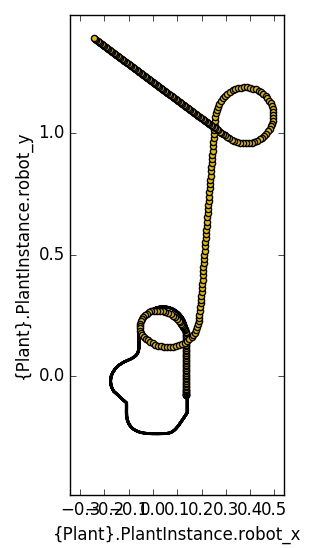
\includegraphics[width=0.5\textwidth]{max_speed_attack.png}
	\caption{Line follower robot path when
	attacked}\label{fig:maxspeedresult}
\end{figure}

In \figref{fig:maxspeedresult} we can see the result of the attack: the FMUs are
activated one at a time, so the robot will turn left since the right FMU is
attacked earlier, then it will go straight, and it will turn right again, since
the right attack FMU stops injecting attack values. In the last part of the
figure we can see the robot going straight, this can be explained looking at the
last legitimate value for the actuators before the attack started.
